% $Author: oscar $
% $Date: 2009-09-15 16:53:48 +0200 (Tue, 15 Sep 2009) $
% $Revision: 29111 $
%=================================================================
\ifx\wholebook\relax\else
% --------------------------------------------
% Lulu:
	\documentclass[a4paper,10pt,twoside]{book}
	\usepackage[
		papersize={6.13in,9.21in},
		hmargin={.815in,.815in},
		vmargin={.98in,.98in},
		ignoreheadfoot
	]{geometry}
	% $Author: oscar $
% $Date: 2009-09-13 20:58:29 +0200 (Sun, 13 Sep 2009) $
% $Revision: 29070 $
%=============================================================
% NB: documentclass must be set in main document.
% Allows book to be generated in multiple formats.
%=============================================================
%:Packages
\usepackage[T1]{fontenc}  %%%%%really important to get the code directly in the text!
\usepackage{palatino}
\usepackage{ifthen}
\usepackage{graphicx}
\graphicspath{{figures/}}
\usepackage{xspace}
\usepackage{makeidx}
\usepackage{isodateo} % enable \isodate
\usepackage{amssymb,textcomp}
%=============================================================
%:More packages
%\usepackage[english]{babel}
%\usepackage{lmodern}
%\usepackage[scaled=0.85]{helvet}
%\usepackage{microtype}
%\usepackage{theorem}
%\usepackage{float}
%\usepackage{longtable}
%\usepackage[nottoc]{tocbibind}
%\usepackage{multicol}
%\usepackage{booktabs}	% book-style tables
%\usepackage{topcapt}	% enables \topcaption
%\usepackage{multirow}
%\usepackage{tabularx}
%\usepackage{alltt}
\usepackage[usenames,dvipsnames]{color}
%\usepackage[hang]{subfigure}\makeatletter\def\p@subfigure{\thefigure\,}\makeatother
%\usepackage{rotating}
%\usepackage{enumitem}	% apb: allows more control over tags in enumerations
%\usepackage{verbatim}     % for comment environment
%\usepackage{varioref}	% for page references that work
%\usepackage{needspace}
%\usepackage[newparttoc]{titlesec}
%\usepackage{titletoc}
%\usepackage{wrapfig}
\usepackage[
	colorlinks=true,
	linkcolor=black,
	urlcolor=black,
	citecolor=black
]{hyperref}   % should come last
%=============================================================
%:URL style
\makeatletter
\def\url@leostyle{%
  \@ifundefined{selectfont}{\def\UrlFont{\sf}}{\def\UrlFont{\sffamily}}}
\makeatother
\urlstyle{leo}
%=============================================================
%:Booleans
\newboolean{lulu}
\setboolean{lulu}{false}
\newcommand{\ifluluelse}[2]{\ifthenelse{\boolean{lulu}}{#1}{#2}}
%=============================================================
%:Editorial comment macros
\newcommand{\nnbb}[2]{
  \fbox{\bfseries\sffamily\scriptsize#1}
  {\sf\small$\blacktriangleright$\textit{#2}$\blacktriangleleft$}
}
\newcommand{\on}[1]{\nnbb{Oscar}{#1}}
\newcommand{\here}{\nnbb{CONTINUE}{HERE}}
%=============================================================
%:Abbreviation macros
\newcommand{\ie}{\emph{i.e.},\xspace}
\newcommand{\eg}{\emph{e.g.},\xspace}
\newcommand{\etc}{\emph{etc.}\xspace}
\newcommand{\etal}{\emph{et al.}\xspace}
\newcommand{\straightquote}{"}
\newcommand{\sba}{\url{SquareBracketAssociates.org}\xspace}
%=============================================================
%:Patterns
% \newcommand{\pattern}[2]{\newpage\section{{\sf #1}}\label{pat:#2}}
% \newcommand{\pattern}[2]{\newpage\index{#1 (Pattern)}\section{#1}\label{pat:#2}}
\newcommand{\pattern}[2]{\cleardoublepage\index{#1 (Pattern)}\section{#1}\label{pat:#2}}
\newcommand{\thumbnail}[2]{\index{#1 (Pattern)}\subsection{#1}\label{pat:#2}}
\newcommand{\thumblang}[2]{\index{#1 (Pattern language)}\subsection{#1}\label{pat:#2}}
\newcommand{\variant}[1]{{\emph{#1}}\xspace}
% \newcommand{\problem}[1]{\subsection*{Problem}\emph{#1}}
\newcommand{\intent}[1]{\paragraph{Intent}\emph{#1}}
\newcommand{\problem}[1]{\paragraph{Problem}\emph{#1}}
\newcommand{\solution}[1]{\paragraph{Solution}\emph{#1}}
\newcommand{\discussion}[0]{\paragraph{Discussion}}
\newcommand{\cmd}[1]{{\tt #1}\xspace}
%=============================================================
%:Environments
\newenvironment{bulletlist}{\begin{itemize}\setlength{\itemsep}{0ex}}
{\end{itemize}}
%=============================================================
%:Cross reference macros
\newcommand{\chalabel}[1]{\label{cha:#1}}
\newcommand{\seclabel}[1]{\label{sec:#1}}
\newcommand{\figlabel}[1]{\label{fig:#1}}
\newcommand{\tablabel}[1]{\label{tab:#1}}
\newcommand{\rulelabel}[1]{\label{rule:#1}}
\newcommand{\eglabel}[1]{\label{eg:#1}}
\newcommand{\scrlabel}[1]{\label{scr:#1}}
\newcommand{\mthlabel}[1]{\label{mth:#1}}
\newcommand{\clslabel}[1]{\label{cls:#1}}
\newcommand{\faqlabel}[1]{\label{faq:#1}}
%\newcommand{\charef}[1]{Chapter~\ref{cha:#1}\xspace}
%\newcommand{\secref}[1]{Section~\ref{sec:#1}\xspace}
\newcommand{\figref}[1]{Figure~\ref{fig:#1}\xspace}
% \newcommand{\patpgref}[2]{\hyperref[pat:#2]{\sf #1} [p.~\pageref{pat:#2}]\xspace}
\newcommand{\patpgref}[2]{\index{#1 (Pattern)}\hyperref[pat:#2]{#1} [p.~\pageref{pat:#2}]\xspace}
\newcommand{\patlangpgref}[2]{\index{#1 (Pattern language)}\hyperref[pat:#2]{#1} [p.~\pageref{pat:#2}]\xspace}
% \newcommand{\patref}[2]{\hyperref[pat:#2]{\sf #1}\xspace}
\newcommand{\patref}[2]{\index{#1 (Pattern)}\hyperref[pat:#2]{#1}\xspace}
\newcommand{\patlangref}[2]{\index{#1 (Pattern language)}\hyperref[pat:#2]{#1}\xspace}
% \newcommand{\charef}[2]{\hyperref[cha:#2]{\underline{\sf #1}}\xspace}
% \newcommand{\charef}[2]{\hyperref[cha:#2]{\sf #1}\xspace}
\newcommand{\charef}[2]{\index{#1 (Pattern cluster)}\hyperref[cha:#2]{#1}\xspace}
% \newcommand{\chapgref}[2]{\hyperref[cha:#2]{\sf #1} [p.~\pageref{cha:#2}]\xspace}
\newcommand{\chapgref}[2]{\index{#1 (Pattern cluster)}\hyperref[cha:#2]{#1} [p.~\pageref{cha:#2}]\xspace}
%\newcommand{\Figref}[1]{Figure~\ref{fig:#1}\xspace}
%\newcommand{\appref}[1]{Appendix~\ref{app:#1}\xspace}
%\newcommand{\tabref}[1]{Table~\ref{tab:#1}\xspace}
%\newcommand{\ruleref}[1]{\ref{rule:#1}\xspace}
%\newcommand{\egref}[1]{example~\ref{eg:#1}\xspace}
%\newcommand{\Egref}[1]{Example~\ref{eg:#1}\xspace}
%\newcommand{\scrref}[1]{script~\ref{scr:#1}\xspace}
%\newcommand{\Scrref}[1]{Script~\ref{scr:#1}\xspace}
%\newcommand{\tscrref}[1]{the script~\ref{scr:#1}\xspace}
%\newcommand{\Tscrref}[1]{The script~\ref{scr:#1}\xspace}
%\newcommand{\mthref}[1]{method~\ref{mth:#1}\xspace}
%\newcommand{\mthsref}[1]{methods~\ref{mth:#1}\xspace}
%\newcommand{\Mthref}[1]{Method~\ref{mth:#1}\xspace}
%\newcommand{\tmthref}[1]{the method~\ref{mth:#1}\xspace}
%\newcommand{\Tmthref}[1]{The method~\ref{mth:#1}\xspace}
%\newcommand{\clsref}[1]{class~\ref{cls:#1}\xspace}
%\newcommand{\tclsref}[1]{the class~\ref{cls:#1}\xspace}
%\newcommand{\Tclsref}[1]{The class~\ref{cls:#1}\xspace}
%=============================================================
%:Page Layout
\setlength{\headsep}{1cm}
%=============================================================
%:Menu item macro
%\definecolor{lightgray}{gray}{0.89}
%\newcommand{\menu}[1]{{%
%	\setlength{\fboxsep}{0pt}%
%	\colorbox{lightgray}{{{\upshape\sffamily\strut \,#1\,}}}}}
%\newcommand{\go}{\,$\triangleright$\,}
%\newcommand{\short}[1]{\mbox{{\sc cmd}\hspace{0.08em}--\hspace{0.09em}#1}\xspace}
%\newcommand{\button}[1]{{%
%	\setlength{\fboxsep}{0pt}%
%	\fbox{{\upshape\sffamily\strut \,#1\,}}}}
%\newcommand{\toolsflap}{\textit{Tools} flap\xspace}
%=============================================================
%:Section depth
%\setcounter{secnumdepth}{2}
%
%\DeclareGraphicsExtensions{.pdf, .jpg, .png}
%=============================================================
%:PDF setup
\hypersetup{
   pdftitle={Object-Oriented Reengineering Patterns},
   pdfauthor={Serge Demeyer, St\'ephane Ducasse, Oscar Nierstrasz},
   pdfkeywords={Reengineering, Object-Oriented Programming, Patterns},
   pdfsubject={Computer Science}
}
%=============================================================
%:Page layout and appearance
%\renewcommand{\chaptermark}[1]{\markboth{#1}{}}
%\renewcommand{\sectionmark}[1]{\markright{\thesection\ #1}}
%\renewpagestyle{plain}[\small\itshape]{%
%	\setheadrule{0pt}%
%	\sethead[][][]{}{}{}%
%	\setfoot[][][]{}{}{}}
%\renewpagestyle{headings}[\small\itshape]{%
%	\setheadrule{0pt}%
%	\setmarks{chapter}{section}%
%	\sethead[\thepage][][\chaptertitle]{\sectiontitle}{}{\thepage}%
%	\setfoot[][][]{}{}{}}
%=============================================================
%:Title section setup and TOC numbering depth
%\setcounter{secnumdepth}{1}
%\setcounter{tocdepth}{1}
%\titleformat{\part}[display]{\centering}{\huge\partname\ \thepart}{1em}{\Huge\textbf}[]
%\titleformat{\chapter}[display]{}{\huge\chaptertitlename\ \thechapter}{1em}{\Huge\raggedright\textbf}[]
%\titlecontents{part}[3pc]{%
%		\pagebreak[2]\addvspace{1em plus.4em minus.2em}%
%		\leavevmode\large\bfseries}
%	{\contentslabel{3pc}}{\hspace*{-3pc}}
%	{}[\nopagebreak]
%\titlecontents{chapter}[3pc]{%
%		\pagebreak[0]\addvspace{1em plus.2em minus.2em}%
%		\leavevmode\bfseries}
%	{\contentslabel{3pc}}{}
%	{\hfill\contentspage}[\nopagebreak]
%\dottedcontents{section}[3pc]{}{3pc}{1pc}
%\dottedcontents{subsection}[3pc]{}{0pc}{1pc}
%\let\origdoublepage\cleardoublepage
%\newcommand{\clearemptydoublepage}{%
%  \clearpage
%  {\pagestyle{empty}\origdoublepage}}
%\let\cleardoublepage\clearemptydoublepage % see http://www.tex.ac.uk/cgi-bin/texfaq2html?label=patch
%=============================================================
%:Listings package configuration
\newcommand{\caret}{\makebox{\raisebox{0.4ex}{\footnotesize{$\wedge$}}}}
% \newcommand{\escape}{{\sf \textbackslash}}
\definecolor{source}{gray}{0.95}
\usepackage{listings}
\lstdefinelanguage{Smalltalk}{
  morestring=[d]',
% Adapt this to other languages!
%  morecomment=[s]{"}{"},
  alsoletter={\#:},
  %escapechar={!},
  literate=
    {BANG}{!}1
%    {UNDERSCORE}{\_}1
    {\\st}{Smalltalk}9 % convenience -- in case \st occurs in code
    % {'}{{\textquotesingle}}1 % replaced by upquote=true in \lstset
%    {_}{{$\leftarrow$}}1
    {>>>}{{\sep}}1
    {^}{{$\uparrow$}}1
    {~}{{$\sim$}}1
    {-}{{\sf -\hspace{-0.13em}-}}1  % the goal is to make - the same width as +
    {+}{\raisebox{0.08ex}{+}}1		% and to raise + off the baseline to match -
    {-->}{{\quad$\longrightarrow$\quad}}3
	, % Don't forget the comma at the end!
  tabsize=4
}[keywords,comments,strings]

\lstset{language=Smalltalk,
	basicstyle=\sffamily,
	keywordstyle=\color{black}\bfseries,
	% stringstyle=\ttfamily, % Ugly! do we really want this? -- on
	mathescape=true,
	showstringspaces=false,
	keepspaces=true,
	breaklines=true,
	breakautoindent=true,
	backgroundcolor=\color{source},
	lineskip={-1pt}, % Ugly hack
	upquote=true, % straight quote; requires textcomp package
	columns=fullflexible} % no fixed width fonts
% \newcommand{\ct}{\lstinline[mathescape=false,basicstyle={\sffamily\upshape}]}
\newcommand{\ct}{\lstinline[mathescape=false,backgroundcolor=\color{white},basicstyle={\sffamily\upshape}]}
\newcommand{\lct}[1]{{\textsf{\textup{#1}}}}
%\newcommand{\scat}[1]{\emph{\textsf{#1}}\xspace}
%\newcommand{\prot}[1]{\emph{\textsf{#1}}\xspace}
% NB: No argument!
\lstnewenvironment{code}[0]{%
	\lstset{%
		% frame=lines,
		frame=single,
		framerule=0pt,
		mathescape=false
	}
}{}
%\def\ignoredollar#1{}
%=============================================================
%:Reserving space
%\newcommand{\needlines}[1]{\Needspace{#1\baselineskip}}
%=============================================================
%:Indexing macros
% Macros ending with "ind" generate text as well as an index entry
% Macros ending with "index" *only* generate an index entry
\newcommand{\ind}[1]{\index{#1}#1\xspace} % plain text
\newcommand{\subind}[2]{\index{#1!#2}#2\xspace} % show #2, subindex under #1
\newcommand{\emphind}[1]{\index{#1}\emph{#1}\xspace} % emph #1
\newcommand{\emphsubind}[2]{\index{#1!#2}\emph{#2}\xspace} % show emph #2, subindex under #1
\newcommand{\patind}[1]{\index{#1@#1 (pattern)}\ct{#1}\xspace} % pattern
\newcommand{\seeindex}[2]{\index{#1|see{#2}}} % #1, see #2
%\newcommand{\boldidx}[1]{{\bf #1}} % breaks hyperlink
%\newcommand{\indmain}[1]{\index{#1}#1\xspace} 
%\newcommand{\emphsubindmain}[2]{\index{#1!#2}\emph{#2}\xspace} % subindex, main entry
%\newcommand{\subindmain}[2]{\index{#1!#2}#2\xspace} % subindex, main entry
%\newcommand{\clsindmain}[1]{\index{#1!\#@(class)}\ct{#1}\xspace} % class main
%\newcommand{\indexmain}[1]{\index{#1}} 
%=============================================================
\parskip 1ex
%=============================================================

	\pagestyle{headings}
	\setboolean{lulu}{true}
% --------------------------------------------
% A4:
%	\documentclass[a4paper,11pt,twoside]{book}
%	% $Author: oscar $
% $Date: 2009-09-13 20:58:29 +0200 (Sun, 13 Sep 2009) $
% $Revision: 29070 $
%=============================================================
% NB: documentclass must be set in main document.
% Allows book to be generated in multiple formats.
%=============================================================
%:Packages
\usepackage[T1]{fontenc}  %%%%%really important to get the code directly in the text!
\usepackage{palatino}
\usepackage{ifthen}
\usepackage{graphicx}
\graphicspath{{figures/}}
\usepackage{xspace}
\usepackage{makeidx}
\usepackage{isodateo} % enable \isodate
\usepackage{amssymb,textcomp}
%=============================================================
%:More packages
%\usepackage[english]{babel}
%\usepackage{lmodern}
%\usepackage[scaled=0.85]{helvet}
%\usepackage{microtype}
%\usepackage{theorem}
%\usepackage{float}
%\usepackage{longtable}
%\usepackage[nottoc]{tocbibind}
%\usepackage{multicol}
%\usepackage{booktabs}	% book-style tables
%\usepackage{topcapt}	% enables \topcaption
%\usepackage{multirow}
%\usepackage{tabularx}
%\usepackage{alltt}
\usepackage[usenames,dvipsnames]{color}
%\usepackage[hang]{subfigure}\makeatletter\def\p@subfigure{\thefigure\,}\makeatother
%\usepackage{rotating}
%\usepackage{enumitem}	% apb: allows more control over tags in enumerations
%\usepackage{verbatim}     % for comment environment
%\usepackage{varioref}	% for page references that work
%\usepackage{needspace}
%\usepackage[newparttoc]{titlesec}
%\usepackage{titletoc}
%\usepackage{wrapfig}
\usepackage[
	colorlinks=true,
	linkcolor=black,
	urlcolor=black,
	citecolor=black
]{hyperref}   % should come last
%=============================================================
%:URL style
\makeatletter
\def\url@leostyle{%
  \@ifundefined{selectfont}{\def\UrlFont{\sf}}{\def\UrlFont{\sffamily}}}
\makeatother
\urlstyle{leo}
%=============================================================
%:Booleans
\newboolean{lulu}
\setboolean{lulu}{false}
\newcommand{\ifluluelse}[2]{\ifthenelse{\boolean{lulu}}{#1}{#2}}
%=============================================================
%:Editorial comment macros
\newcommand{\nnbb}[2]{
  \fbox{\bfseries\sffamily\scriptsize#1}
  {\sf\small$\blacktriangleright$\textit{#2}$\blacktriangleleft$}
}
\newcommand{\on}[1]{\nnbb{Oscar}{#1}}
\newcommand{\here}{\nnbb{CONTINUE}{HERE}}
%=============================================================
%:Abbreviation macros
\newcommand{\ie}{\emph{i.e.},\xspace}
\newcommand{\eg}{\emph{e.g.},\xspace}
\newcommand{\etc}{\emph{etc.}\xspace}
\newcommand{\etal}{\emph{et al.}\xspace}
\newcommand{\straightquote}{"}
\newcommand{\sba}{\url{SquareBracketAssociates.org}\xspace}
%=============================================================
%:Patterns
% \newcommand{\pattern}[2]{\newpage\section{{\sf #1}}\label{pat:#2}}
% \newcommand{\pattern}[2]{\newpage\index{#1 (Pattern)}\section{#1}\label{pat:#2}}
\newcommand{\pattern}[2]{\cleardoublepage\index{#1 (Pattern)}\section{#1}\label{pat:#2}}
\newcommand{\thumbnail}[2]{\index{#1 (Pattern)}\subsection{#1}\label{pat:#2}}
\newcommand{\thumblang}[2]{\index{#1 (Pattern language)}\subsection{#1}\label{pat:#2}}
\newcommand{\variant}[1]{{\emph{#1}}\xspace}
% \newcommand{\problem}[1]{\subsection*{Problem}\emph{#1}}
\newcommand{\intent}[1]{\paragraph{Intent}\emph{#1}}
\newcommand{\problem}[1]{\paragraph{Problem}\emph{#1}}
\newcommand{\solution}[1]{\paragraph{Solution}\emph{#1}}
\newcommand{\discussion}[0]{\paragraph{Discussion}}
\newcommand{\cmd}[1]{{\tt #1}\xspace}
%=============================================================
%:Environments
\newenvironment{bulletlist}{\begin{itemize}\setlength{\itemsep}{0ex}}
{\end{itemize}}
%=============================================================
%:Cross reference macros
\newcommand{\chalabel}[1]{\label{cha:#1}}
\newcommand{\seclabel}[1]{\label{sec:#1}}
\newcommand{\figlabel}[1]{\label{fig:#1}}
\newcommand{\tablabel}[1]{\label{tab:#1}}
\newcommand{\rulelabel}[1]{\label{rule:#1}}
\newcommand{\eglabel}[1]{\label{eg:#1}}
\newcommand{\scrlabel}[1]{\label{scr:#1}}
\newcommand{\mthlabel}[1]{\label{mth:#1}}
\newcommand{\clslabel}[1]{\label{cls:#1}}
\newcommand{\faqlabel}[1]{\label{faq:#1}}
%\newcommand{\charef}[1]{Chapter~\ref{cha:#1}\xspace}
%\newcommand{\secref}[1]{Section~\ref{sec:#1}\xspace}
\newcommand{\figref}[1]{Figure~\ref{fig:#1}\xspace}
% \newcommand{\patpgref}[2]{\hyperref[pat:#2]{\sf #1} [p.~\pageref{pat:#2}]\xspace}
\newcommand{\patpgref}[2]{\index{#1 (Pattern)}\hyperref[pat:#2]{#1} [p.~\pageref{pat:#2}]\xspace}
\newcommand{\patlangpgref}[2]{\index{#1 (Pattern language)}\hyperref[pat:#2]{#1} [p.~\pageref{pat:#2}]\xspace}
% \newcommand{\patref}[2]{\hyperref[pat:#2]{\sf #1}\xspace}
\newcommand{\patref}[2]{\index{#1 (Pattern)}\hyperref[pat:#2]{#1}\xspace}
\newcommand{\patlangref}[2]{\index{#1 (Pattern language)}\hyperref[pat:#2]{#1}\xspace}
% \newcommand{\charef}[2]{\hyperref[cha:#2]{\underline{\sf #1}}\xspace}
% \newcommand{\charef}[2]{\hyperref[cha:#2]{\sf #1}\xspace}
\newcommand{\charef}[2]{\index{#1 (Pattern cluster)}\hyperref[cha:#2]{#1}\xspace}
% \newcommand{\chapgref}[2]{\hyperref[cha:#2]{\sf #1} [p.~\pageref{cha:#2}]\xspace}
\newcommand{\chapgref}[2]{\index{#1 (Pattern cluster)}\hyperref[cha:#2]{#1} [p.~\pageref{cha:#2}]\xspace}
%\newcommand{\Figref}[1]{Figure~\ref{fig:#1}\xspace}
%\newcommand{\appref}[1]{Appendix~\ref{app:#1}\xspace}
%\newcommand{\tabref}[1]{Table~\ref{tab:#1}\xspace}
%\newcommand{\ruleref}[1]{\ref{rule:#1}\xspace}
%\newcommand{\egref}[1]{example~\ref{eg:#1}\xspace}
%\newcommand{\Egref}[1]{Example~\ref{eg:#1}\xspace}
%\newcommand{\scrref}[1]{script~\ref{scr:#1}\xspace}
%\newcommand{\Scrref}[1]{Script~\ref{scr:#1}\xspace}
%\newcommand{\tscrref}[1]{the script~\ref{scr:#1}\xspace}
%\newcommand{\Tscrref}[1]{The script~\ref{scr:#1}\xspace}
%\newcommand{\mthref}[1]{method~\ref{mth:#1}\xspace}
%\newcommand{\mthsref}[1]{methods~\ref{mth:#1}\xspace}
%\newcommand{\Mthref}[1]{Method~\ref{mth:#1}\xspace}
%\newcommand{\tmthref}[1]{the method~\ref{mth:#1}\xspace}
%\newcommand{\Tmthref}[1]{The method~\ref{mth:#1}\xspace}
%\newcommand{\clsref}[1]{class~\ref{cls:#1}\xspace}
%\newcommand{\tclsref}[1]{the class~\ref{cls:#1}\xspace}
%\newcommand{\Tclsref}[1]{The class~\ref{cls:#1}\xspace}
%=============================================================
%:Page Layout
\setlength{\headsep}{1cm}
%=============================================================
%:Menu item macro
%\definecolor{lightgray}{gray}{0.89}
%\newcommand{\menu}[1]{{%
%	\setlength{\fboxsep}{0pt}%
%	\colorbox{lightgray}{{{\upshape\sffamily\strut \,#1\,}}}}}
%\newcommand{\go}{\,$\triangleright$\,}
%\newcommand{\short}[1]{\mbox{{\sc cmd}\hspace{0.08em}--\hspace{0.09em}#1}\xspace}
%\newcommand{\button}[1]{{%
%	\setlength{\fboxsep}{0pt}%
%	\fbox{{\upshape\sffamily\strut \,#1\,}}}}
%\newcommand{\toolsflap}{\textit{Tools} flap\xspace}
%=============================================================
%:Section depth
%\setcounter{secnumdepth}{2}
%
%\DeclareGraphicsExtensions{.pdf, .jpg, .png}
%=============================================================
%:PDF setup
\hypersetup{
   pdftitle={Object-Oriented Reengineering Patterns},
   pdfauthor={Serge Demeyer, St\'ephane Ducasse, Oscar Nierstrasz},
   pdfkeywords={Reengineering, Object-Oriented Programming, Patterns},
   pdfsubject={Computer Science}
}
%=============================================================
%:Page layout and appearance
%\renewcommand{\chaptermark}[1]{\markboth{#1}{}}
%\renewcommand{\sectionmark}[1]{\markright{\thesection\ #1}}
%\renewpagestyle{plain}[\small\itshape]{%
%	\setheadrule{0pt}%
%	\sethead[][][]{}{}{}%
%	\setfoot[][][]{}{}{}}
%\renewpagestyle{headings}[\small\itshape]{%
%	\setheadrule{0pt}%
%	\setmarks{chapter}{section}%
%	\sethead[\thepage][][\chaptertitle]{\sectiontitle}{}{\thepage}%
%	\setfoot[][][]{}{}{}}
%=============================================================
%:Title section setup and TOC numbering depth
%\setcounter{secnumdepth}{1}
%\setcounter{tocdepth}{1}
%\titleformat{\part}[display]{\centering}{\huge\partname\ \thepart}{1em}{\Huge\textbf}[]
%\titleformat{\chapter}[display]{}{\huge\chaptertitlename\ \thechapter}{1em}{\Huge\raggedright\textbf}[]
%\titlecontents{part}[3pc]{%
%		\pagebreak[2]\addvspace{1em plus.4em minus.2em}%
%		\leavevmode\large\bfseries}
%	{\contentslabel{3pc}}{\hspace*{-3pc}}
%	{}[\nopagebreak]
%\titlecontents{chapter}[3pc]{%
%		\pagebreak[0]\addvspace{1em plus.2em minus.2em}%
%		\leavevmode\bfseries}
%	{\contentslabel{3pc}}{}
%	{\hfill\contentspage}[\nopagebreak]
%\dottedcontents{section}[3pc]{}{3pc}{1pc}
%\dottedcontents{subsection}[3pc]{}{0pc}{1pc}
%\let\origdoublepage\cleardoublepage
%\newcommand{\clearemptydoublepage}{%
%  \clearpage
%  {\pagestyle{empty}\origdoublepage}}
%\let\cleardoublepage\clearemptydoublepage % see http://www.tex.ac.uk/cgi-bin/texfaq2html?label=patch
%=============================================================
%:Listings package configuration
\newcommand{\caret}{\makebox{\raisebox{0.4ex}{\footnotesize{$\wedge$}}}}
% \newcommand{\escape}{{\sf \textbackslash}}
\definecolor{source}{gray}{0.95}
\usepackage{listings}
\lstdefinelanguage{Smalltalk}{
  morestring=[d]',
% Adapt this to other languages!
%  morecomment=[s]{"}{"},
  alsoletter={\#:},
  %escapechar={!},
  literate=
    {BANG}{!}1
%    {UNDERSCORE}{\_}1
    {\\st}{Smalltalk}9 % convenience -- in case \st occurs in code
    % {'}{{\textquotesingle}}1 % replaced by upquote=true in \lstset
%    {_}{{$\leftarrow$}}1
    {>>>}{{\sep}}1
    {^}{{$\uparrow$}}1
    {~}{{$\sim$}}1
    {-}{{\sf -\hspace{-0.13em}-}}1  % the goal is to make - the same width as +
    {+}{\raisebox{0.08ex}{+}}1		% and to raise + off the baseline to match -
    {-->}{{\quad$\longrightarrow$\quad}}3
	, % Don't forget the comma at the end!
  tabsize=4
}[keywords,comments,strings]

\lstset{language=Smalltalk,
	basicstyle=\sffamily,
	keywordstyle=\color{black}\bfseries,
	% stringstyle=\ttfamily, % Ugly! do we really want this? -- on
	mathescape=true,
	showstringspaces=false,
	keepspaces=true,
	breaklines=true,
	breakautoindent=true,
	backgroundcolor=\color{source},
	lineskip={-1pt}, % Ugly hack
	upquote=true, % straight quote; requires textcomp package
	columns=fullflexible} % no fixed width fonts
% \newcommand{\ct}{\lstinline[mathescape=false,basicstyle={\sffamily\upshape}]}
\newcommand{\ct}{\lstinline[mathescape=false,backgroundcolor=\color{white},basicstyle={\sffamily\upshape}]}
\newcommand{\lct}[1]{{\textsf{\textup{#1}}}}
%\newcommand{\scat}[1]{\emph{\textsf{#1}}\xspace}
%\newcommand{\prot}[1]{\emph{\textsf{#1}}\xspace}
% NB: No argument!
\lstnewenvironment{code}[0]{%
	\lstset{%
		% frame=lines,
		frame=single,
		framerule=0pt,
		mathescape=false
	}
}{}
%\def\ignoredollar#1{}
%=============================================================
%:Reserving space
%\newcommand{\needlines}[1]{\Needspace{#1\baselineskip}}
%=============================================================
%:Indexing macros
% Macros ending with "ind" generate text as well as an index entry
% Macros ending with "index" *only* generate an index entry
\newcommand{\ind}[1]{\index{#1}#1\xspace} % plain text
\newcommand{\subind}[2]{\index{#1!#2}#2\xspace} % show #2, subindex under #1
\newcommand{\emphind}[1]{\index{#1}\emph{#1}\xspace} % emph #1
\newcommand{\emphsubind}[2]{\index{#1!#2}\emph{#2}\xspace} % show emph #2, subindex under #1
\newcommand{\patind}[1]{\index{#1@#1 (pattern)}\ct{#1}\xspace} % pattern
\newcommand{\seeindex}[2]{\index{#1|see{#2}}} % #1, see #2
%\newcommand{\boldidx}[1]{{\bf #1}} % breaks hyperlink
%\newcommand{\indmain}[1]{\index{#1}#1\xspace} 
%\newcommand{\emphsubindmain}[2]{\index{#1!#2}\emph{#2}\xspace} % subindex, main entry
%\newcommand{\subindmain}[2]{\index{#1!#2}#2\xspace} % subindex, main entry
%\newcommand{\clsindmain}[1]{\index{#1!\#@(class)}\ct{#1}\xspace} % class main
%\newcommand{\indexmain}[1]{\index{#1}} 
%=============================================================
\parskip 1ex
%=============================================================

%	\usepackage{a4wide}
% --------------------------------------------
	\begin{document}
	\renewcommand{\nnbb}[2]{} % Disable editorial comments
	\sloppy
\fi
%=================================================================
\chapter{Migration Strategies}
\chalabel{MigrationStrategies}

\on{Put these in the right places:}

\label{pat:AlwaysHaveARunningVersion}

Your reengineering project is well underway. You have developed a good understanding of the legacy system and you have started to \patpgref{Write Tests to Enable Evolution}{WriteTestsToEnableEvolution}. You have gone through a process of \charef{Setting Direction}{SettingDirection} and have decided to tackle the \patpgref{Most Valuable First}{MostValuableFirst}.

How can you be sure that the new system will be accepted by users? How do you migrate to the new system while the old system is being used? How can you test and evaluate the new system before it is finished?

\subsection*{Forces}

\begin{bulletlist}
\item Big-bang migration carries a high risk of failure.

\item Introducing too many changes at once may alienate users.

\item Constant feedback helps you stay on track, though it may be difficult and costly to achieve.

\item Users have to get their work done; they don't want to be distracted by incomplete solution.

\item Legacy data must survive while the system is being used.
\end{bulletlist}

\subsection*{Overview}

It is not enough to reengineer a legacy system and then deploy it. In fact, if you try this, you will surely fail (for the same reasons that big Waterfall projects in new territories often fail). You must be prepared to introduce the new solution gradually, to gain the confidence and collaboration of the users, and you must adopt a strategy for migrating gradually and painlessly from the existing system, \emph{while it is still being deployed}, to the new system.

\begin{figure}
\begin{center}
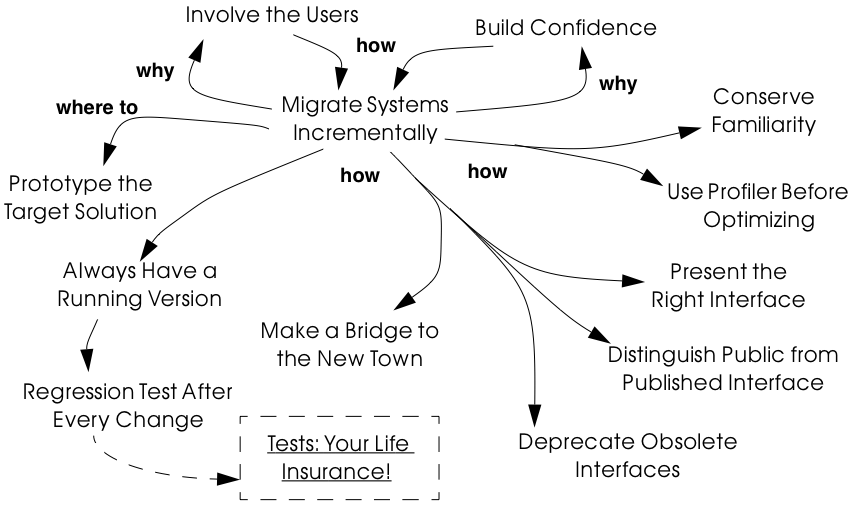
\includegraphics[width=\textwidth]{MigrationMap}
\caption{How, why and whither to migrate legacy systems.}
\figlabel{MigrationMap}
\end{center}
\end{figure}

The central message of this cluster is to \patref{Migrate Systems Incrementally}{MigrateSystemsIncrementally}. This is, however, easier said than done. In figure 25 we can see that in order to \patref{Migrate Systems Incrementally}{MigrateSystemsIncrementally}, we should consider a large number of other patterns. Since there exists a vast literature on system migration, we do not attempt to cover the topic in great detail. We have selected, however, the patterns that we consider to be most important for reengineering object-oriented legacy systems, and summarized the main points. Where appropriate, we point the reader to further sources of information.

Although the central pattern of this cluster is \patref{Migrate Systems Incrementally}{MigrateSystemsIncrementally}, the key motivation is provided by \patref{Involve the Users}{InvolveTheUsers} and \patref{Build Confidence}{BuildConfidence}. These first three patterns are fundamental patterns for minimizing risk and increasing the chances of success:

\begin{bulletlist}
\item \patref{Involve the Users}{InvolveTheUsers} increases the chance that users will accept the new system by involving them closely in the entire reengineering process, getting them to use intermediate results, and providing them with strong support. It is easier to achieve if you \patref{Migrate Systems Incrementally}{MigrateSystemsIncrementally} and \patref{Build Confidence}{BuildConfidence} step by step.

\item \patref{Build Confidence}{BuildConfidence} helps you overcome skepticism and doubt by regularly delivering results that are of value to the users. 

\item \patref{Migrate Systems Incrementally}{MigrateSystemsIncrementally} recommends that the old system be gradually and incrementally replaced by the new system. New results can then be integrated as you proceed, thus helping you to \patref{Build Confidence}{BuildConfidence} and \patref{Involve the Users}{InvolveTheUsers}.
\end{bulletlist}

It is very hard to \patref{Migrate Systems Incrementally}{MigrateSystemsIncrementally} unless you also adhere to the following practices:

\begin{bulletlist}
\item \patref{Prototype the Target Solution}{PrototypeTheTargetSolution} to test the new architecture and new technical risks. It is too easy to be tempted to think you don't need a prototype since you already have a running system, but this is almost always a mistake.

\item \patref{Always Have a Running Version}{AlwaysHaveARunningVersion} helps to keep changes in sync by ensuring that they are integrated frequently.

\item \patref{Regression Test After Every Change}{RegressionTestAfterEveryChange} helps to you \patref{Always Have a Running Version}{AlwaysHaveARunningVersion} by making sure that everything that used to run still runs. It presupposes that you \patpgref{Write Tests to Enable Evolution}{WriteTestsToEnableEvolution}.
\end{bulletlist}

Depending on the circumstances, there are various practices that may help you to \patref{Migrate Systems Incrementally}{MigrateSystemsIncrementally}:

\begin{bulletlist}
\item \patref{Make a Bridge to the New Town}{MakeABridgeToTheNewTown} introduces the metaphor of a (data) ``bridge'' to allow you to gradually migrate data from a legacy component to its replacement, while the two run in tandem. When all the data have been transferred, the legacy component can be retired.

\item \patref{Present the Right Interface}{PresentTheRightInterface} helps you to develop the target system in increments by wrapping the old functionality to export the abstractions you really want.

\item \patref{Distinguish Public from Published Interface}{DistinguishPublicFromPublishedInterface} distinguishes between stable (public) and unstable (published) interfaces to facilitate parallel development within a reengineering team.

\item \patref{Deprecate Obsolete Interfaces}{DeprecateObsoleteInterfaces} lets you gracefully retire obsolete interfaces without immediately invalidating clients.
\end{bulletlist}

Finally, the following two practices may help you avoid making radical, but unnecessary changes:

\begin{bulletlist}
\item \patref{Conserve Familiarity}{ConserveFamiliarity} warns you against introducing radical interface changes that may alienate users.

\item \patpgref{Use Profiler Before Optimizing}{UseProfilerBeforeOptimizing} reminds you to delay considering performance issues until you can demonstrate that you have a problem and can pinpoint the source of the problem.
\end{bulletlist}

%=================================================================
%:PATTERN -- {Involve the Users}
\pattern{Involve the Users}{InvolveTheUsers}


\emph{Also Known As:}  \ind{Engage Customers} \cite{Copl95d}

\intent{Maximize acceptance of changes by involving the users at every step.}

\subsection*{Problem}

How can you be sure that users will accept the reengineered system?

\emph{This problem is difficult because:} 

\begin{bulletlist}
\item The old systems works. It is clunky, but the users know how it works and know how to get around the problems.

\item People hate to have to learn something new unless it really makes their life simpler.

\item User perceptions of what is needed to improve a system tend to change as the system evolves.

\item Users can have difficulty evaluating a paper design.

\item It is hard to get excited about a new system that is not ready to use.
\end{bulletlist}

\emph{Yet, solving this problem is feasible because:}

\begin{bulletlist}
\item Users will try new solutions if they see that their needs are being seriously addressed.

\item Users will give you feedback if you give them something useful to use.
\end{bulletlist}

\subsection*{Solution}

Get the users directly involved in the new development, and support them closely in using the new system.

\subsubsection*{Steps}

Get the users to tell you where their priorities lie. Start with \patpgref{Most Valuable First}{MostValuableFirst}. Break the priorities down into small steps that can be delivered in regular increments, so you can \patpgref{Build Confidence}{BuildConfidence}.

Create an environment that will encourage contact between users and developers. Physical location is important.

Establish simple procedures for delivering intermediate results on a regular basis and obtaining feedback. Early prototypes may help, especially to evaluate risky new technologies or approaches. A good strategy is to \patpgref{Migrate Systems Incrementally}{MigrateSystemsIncrementally} so that users can start using the new system as it is being built. You should \patpgref{Conserve Familiarity}{ConserveFamiliarity} to avoid alienating users.

\subsection*{Tradeoffs}

\subsubsection*{Pros}

\begin{bulletlist}
\item Requirements will continuously be validated and updated, increasing your chances that you will move in the right direction.

\item If the users feel they are getting useful results and they are being supported, they will put extra effort into giving useful feedback.

\item Users will be involved throughout the effort, eliminating the need for a special training session late in the project.
\end{bulletlist}

\subsubsection*{Cons}

\begin{bulletlist}
\item Developers may feel that supporting users is distracting them from the job of reengineering the system.

\index{Yourdon, Edward}
\item If you succeed in involving the users, this will raise expectations and put extra pressure on your team. For instance, Yourdon mentions that prototypes can really raise expectations too much and that you should always make clear which parts are not yet working \cite{Your97a}.
\end{bulletlist}

\subsubsection*{Difficulties}

\begin{bulletlist}
\item It can be hard to involve the users initially, before you have shown any results.

\item You can't involve everybody, and the users who are left out might feel neglected.
\end{bulletlist}

\subsection*{Rationale}

You need a feedback loop to ensure that you are addressing the real customer needs. By involving and supporting the users, you encourage this feedback loop.

\index{Coplien, James}
Coplien points out: \emph{``Note that `maintaining product quality' is not the problem being solved here. Product quality is only one component of customer satisfaction.''} \cite{Copl95d}

\subsection*{Related Patterns}

Virtually all of the patterns in this cluster support \patref{Involve the Users}{InvolveTheUsers}. \patref{Migrate Systems Incrementally}{MigrateSystemsIncrementally} to get the users working with the system as it is being reengineered and thereby \patref{Build Confidence}{BuildConfidence}.

The \ind{Planning Game} \cite{Beck01a} is an effective technique to \patref{Involve the Users}{InvolveTheUsers} by iteratively identifying stories, estimating costs, and committing to the stories to be released.

%=================================================================
%:PATTERN -- {Build Confidence}
\pattern{Build Confidence}{BuildConfidence}


\intent{Improve your chances of overall success by demonstrating results in regular increments.}

\subsection*{Problem}

How can you overcome the high degree of skepticism that customers and team members often have for any kind of software project?

\emph{This problem is difficult because:} 

\begin{bulletlist}
\item Few software projects meet requirements, come in on time, and stay within budget. The skepticism that accompanies most projects can easily lead to defeatism, and projects can fail as a self-fulfilling prophecy.

\item Users rarely get what they really want or need.

\item It can be hard to convince either the users or even your own team that the legacy system can really be salvaged.
\end{bulletlist}

\emph{Yet, solving this problem is feasible because:}

\begin{bulletlist}
\item You don't need to solve all the problems at once.
\end{bulletlist}

\subsection*{Solution}

Create a positive atmosphere by demonstrating some positive results as early as you can, and continue to do so on a regular basis.

\subsubsection*{Steps}

Pick short intervals for delivering new results. At each step, try to agree together with the users what are the smallest results that can demonstrate real value.

\subsection*{Tradeoffs}

\subsubsection*{Pros}

\begin{bulletlist}
\item Both users and developers can measure real progress.

\item It is easier to estimate the cost of smaller steps.
\end{bulletlist}

\subsubsection*{Cons}

\begin{bulletlist}
\item It takes time to frequently synchronize with the users.

\item Users may resent the extra work it takes to use the new system in tandem with the old one.

\item If you succeed to demonstrate good results early in the project, you may raise expectations too high.
\end{bulletlist}

\subsubsection*{Difficulties}

\begin{bulletlist}
\item Some requirements can be hard to break down into small steps, particularly if they entail architectural changes to the system.

\item Reengineering teams must be careful not to alienate the developers of the original system, since they are one of the most valuable sources of information.

\item It is not enough to convince users --- you must also take care to get commitment from management. It is hard to convince management in small steps. Plan big demos at regular intervals.
\end{bulletlist}

\subsection*{Rationale}

By taking smaller steps, you reduce the risk that an individual step will fail. Frequent, positive results help to build confidence. By the same token, \ind{Extreme Programming} advocates \ind{Small Releases} \cite{Beck00a}. Even negative results help you to monitor progress and understand better the situation, and so help to build up confidence.

\subsection*{Related Patterns}

\patref{Prototype the Target Solution}{PrototypeTheTargetSolution} and \patref{Make a Bridge to the New Town}{MakeABridgeToTheNewTown} can make it easier to demonstrate results in small steps. 

It is easier to \patref{Build Confidence}{BuildConfidence} if you \patref{Involve the Users}{InvolveTheUsers}. 

%=================================================================
%:PATTERN -- {Migrate Systems Incrementally}
\pattern{Migrate Systems Incrementally}{MigrateSystemsIncrementally}

\emph{Also Known As:}  \ind{Chicken Little} \cite{Brod95a}

\intent{Avoid complexity and risk of big-bang reengineering by deploying functionality in frequent increments.}

\subsection*{Problem}

When should you plan to deploy the new system?

\emph{This problem is difficult because:} 

\begin{bulletlist}
\item Projects are often planned and funded on large time scales, with ``big bang'' requirements specification done up front.

\item The real requirements are often only clear in hindsight. Users will resist adopting a new system that is radically different from what they are used to, especially if it does not work flawlessly from the beginning.

\item The longer you wait to deploy the new system, the longer you must wait to get user feedback.

\item You cannot deploy an incomplete system. Users do not have time to waste on incomplete solutions.
\end{bulletlist}

\emph{Yet, solving this problem is feasible because:}

\begin{bulletlist}
\item You have a running system that can be extended and modified.
\end{bulletlist}

\subsection*{Solution}

Deploy a first \emph{update} of the legacy system as soon as you can, and migrate incrementally to the target system.

\subsubsection*{Steps}

\begin{bulletlist}
\item Decompose the legacy system into parts.

\item Choose one part to tackle at a time.

\item Put tests in place for that part and the parts that depend on it.

\item Take appropriate steps to wrap, reengineer or replace the legacy component.

\item Deploy the updated component and obtain feedback.

\item Iterate.
\end{bulletlist}

\subsection*{Tradeoffs}

\subsubsection*{Pros}

\begin{bulletlist}
\item You get user feedback early and \patref{Build Confidence}{BuildConfidence}.

\item You see immediately when things break.

\item Users learn the new system as it's being built.

\item The system is always deployed.

\item The system is always being tested, so you can't skip testing.
\end{bulletlist}

\subsubsection*{Cons}

\begin{bulletlist}
\item You will have to work harder to keep the system running while you are changing it.
\end{bulletlist}

\subsubsection*{Difficulties}

\begin{bulletlist}
\item It can be difficult to migrate to a new architecture. You may want to \patref{Prototype the Target Solution}{PrototypeTheTargetSolution} to get the new architecture in place, and \patref{Present the Right Interface}{PresentTheRightInterface} to the old system to hide the legacy interfaces while you migrate the underlying components.

\item It is risky to change a running system. Be sure to \patref{Regression Test After Every Change}{RegressionTestAfterEveryChange}. 
\end{bulletlist}

\subsection*{Rationale}

You get the best user feedback from a running system. Users are more motivated and involved with a system they use daily.

\subsection*{Known Uses}

\emphind{Migrating Legacy Systems} \cite{Brod95a} introduces this pattern under the name ``\ind{Chicken Little}'' (to migrate incrementally means to ``take Chicken Little steps''). This book discusses in great detail strategies and techniques for incremental migration.

\subsection*{Related Patterns}

Apply \patpgref{Most Valuable First}{MostValuableFirst} to select the legacy components to work on first. \patpgref{Appoint a Navigator}{AppointANavigator} to maintain architectural integrity. 

\patpgref{Write Tests to Enable Evolution}{WriteTestsToEnableEvolution}, and \patpgref{Grow Your Test Base Incrementally}{GrowYourTestBaseIncrementally} as you migrate. Be sure to \patpgref{Test the Interface, Not the Implementation}{TestTheInterfaceNotTheImplementation} so you do not always have to rewrite your tests as you reengineer or replace legacy components. \patpgref{Regression Test After Every Change}{RegressionTestAfterEveryChange} so you can \patpgref{Always Have a Running Version}{AlwaysHaveARunningVersion}.

Consider applying \patref{Present the Right Interface}{PresentTheRightInterface} for legacy components that you do not intend to reengineer or replace.

You might consider to \patpgref{Make a Bridge to the New Town}{MakeABridgeToTheNewTown} if you need to migrate data from legacy components that you are replacing.

%=================================================================
%:PATTERN -- {Prototype the Target Solution}
\pattern{Prototype the Target Solution}{PrototypeTheTargetSolution}


\intent{Evaluate the risk of migrating to a new target solution by building a prototype.}

\subsection*{Problem}

How do you know if your ideas for the new target system will work?

\emph{This problem is difficult because:} 

\begin{bulletlist}
\item It is risky to make radical changes to a working system.

\item It can be hard to anticipate how design changes will impact existing functionality.

\item A solution that works is more believable than one that one that has not been tested.
\end{bulletlist}

\emph{Yet, solving this problem is feasible because:}

\begin{bulletlist}
\item You don't need to reengineer the whole legacy system to test the new ideas.
\end{bulletlist}

\subsection*{Solution}

Develop a prototype of the new concept and evaluate it with respect to the new, emerging requirements.

\subsubsection*{Steps}

\begin{bulletlist}
\item Identify the biggest technical risks for your reengineering project. Typically they will concern things like:

\begin{bulletlist}
\item choice of a new system architecture
\item migration of legacy data to new system
\item adequate performance --- or performance gains --- with new technology or platform (for example, demonstrating that a certain transaction throughput can be achieved)
\end{bulletlist}

\index{throwaway prototype}
\index{exploratory prototype}
\index{evolutionary prototype}
\item Decide whether to implement an exploratory (\ie throwaway) prototype that will service purely to evaluate the feasibility of a technical option, or rather an evolutionary prototype that will eventually evolve into the new target system.

\begin{bulletlist}
\item An exploratory prototype must be designed to answer very precise questions. These may be purely technical questions, such as whether the new platform can meet performance constraints set by the legacy system, or they may be usability questions which require participation of and evaluation by the users. The exploratory prototype does not need to be designed to address any other issues or questions, and will not be part of the migrated system (although the answers it provides will influence the new system).

\item An evolutionary prototype, on the other hand, is intended to eventually replace a legacy component, and must therefore reflect the target architecture. The new architecture most not only adequately support the legacy services, but also overcome the obstacles that limit the legacy solution's usefulness. The prototype must be design to answer these risks first.
\end{bulletlist}
\end{bulletlist}

\subsection*{Tradeoffs}

\subsubsection*{Pros}

\begin{bulletlist}
\item A prototype can be built quickly, since it does not have to implement all the functionality of the legacy system.

\item You can hack parts of the legacy system to get your prototype running.

\item You can learn quickly if your ideas for the target system are sound.
\end{bulletlist}

\subsubsection*{Cons}

\begin{bulletlist}
\item Users may not be highly motivated to spend a lot of time evaluating a throwaway prototype.

\item You may be tempted to continue to develop the throwaway prototype.
\end{bulletlist}

\subsubsection*{Difficulties}

\begin{bulletlist}
\item It may be hard to convince yourself or your customer of the need for a prototype --- after all, you already have a running system.

\item It can take too much time to get an evolutionary prototype up to speed. Consider applying \patref{Present the Right Interface}{PresentTheRightInterface} to legacy components to provide a good interface for legacy services to the prototype. 
\end{bulletlist}

\subsection*{Rationale}

\index{Brooks, Frederick}
A prototype can tell you quickly whether a certain technical approach is sound or not. Brooks in \emph{The Mythical Man-Month} \cite{Broo75a} advises us to ``write one to throw away'' since it is hard to get it right the first time.

\index{Love, Tom}
\index{Foote, Brian}
\index{Yoder, Joseph}
Love \cite{Love93a} takes this one step further and warns us that, for object-oriented systems we should ``write two to throw away"! Foote and Yoder \cite{Foot00a} argue that, among other things, \ind{Throwaway Code} is often the best way to clarify domain requirements, but they also warn that a prototype risks evolving into a ``\ind{Big Ball of Mud}''.

\subsection*{Related Patterns}

You might consider applying \patref{Make a Bridge to the New Town}{MakeABridgeToTheNewTown} to migrate legacy data to an evolutionary prototype.

%=================================================================
%:PATTERN -- {Always Have a Running Version}
\pattern{Always Have a Running Version}{AlwaysHaveARunningVersion}


\intent{Increase confidence in changes by regularly rebuilding the system.}

\subsection*{Problem}

How do you convince your customer that you are on the right path?

\emph{This problem is difficult because:} 

\begin{bulletlist}
\item It can be hard to demo a software system under development, or to discuss problems with users since there is often no stable, running version of the system available.

\item Integrating changes from multiple versions of a system can be slow and painful.
\end{bulletlist}

\emph{Yet, solving this problem is feasible because:}

\begin{bulletlist}
\item You don't have to wait until a component is ``finished'' before integrating it.
\end{bulletlist}

\subsection*{Solution}

Institute a discipline of integrating new changes and developments on a daily basis.

\subsubsection*{Steps}

\begin{bulletlist}
\item Have version management and configuration management systems in place.

\item Make sure you have regression tests in place for the parts you are working on.

\item Institute a discipline of short transactions for checking out system components and checking them back in again. Plan iterations to be as short as possible to allow changes to be integrated into a running system.
\end{bulletlist}

\subsection*{Tradeoffs}

\subsubsection*{Pros}

\begin{bulletlist}
\item You always have a working version to demo.

\item You can always have a working version to run your regression tests.

\item You can quickly validate your changes, thereby helping you to \patref{Build Confidence}{BuildConfidence}.
\end{bulletlist}

\subsubsection*{Cons}

\begin{bulletlist}
\item You must continuously integrate changes.
\end{bulletlist}

\subsubsection*{Difficulties}

\begin{bulletlist}
\item Large systems may have very long build times. You may need to rearchitect the system first to enable shorter build times.

\item It can be hard to break some kinds of large modifications into meaningful updates that can be individually integrated. 
\end{bulletlist}

\subsection*{Rationale}

Many practitioners advocate a process of continuous integration as a way to avoid a risky and painful big-bang integration \cite{Booc94a}.

\subsection*{Related Patterns}

\patref{Regression Test After Every Change}{RegressionTestAfterEveryChange} minimizes the risk of defects creeping in during integration. 

\ind{Continuous Integration} \cite{Booc94a} \cite{Beck00a} is a proven way to \patref{Always Have a Running Version}{AlwaysHaveARunningVersion}.

%=================================================================
%:PATTERN -- {Regression Test After Every Change}
\pattern{Regression Test After Every Change}{RegressionTestAfterEveryChange}


\intent{Build confidence by making sure that whatever worked before still works.}

\subsection*{Problem}

How can you be sure that the last change you made won't break the system?

\emph{This problem is difficult because:} 

\begin{bulletlist}
\item In a complex system, small changes can have unexpected side effects. A seemingly innocuous change may break something without this being immediately discovered.
\end{bulletlist}

\emph{Yet, solving this problem is feasible because:}

\begin{bulletlist}
\item You have written test suites that express how the system should behave.
\end{bulletlist}

\subsection*{Solution}

Run your regression test suite every time you think you have reached a stable state.

\subsection*{Tradeoffs}

\subsubsection*{Pros}

\begin{bulletlist}
\item It is easier to \patref{Always Have a Running Version}{AlwaysHaveARunningVersion}.

\item It is easier to \patref{Build Confidence}{BuildConfidence} as you proceed.
\end{bulletlist}

\subsubsection*{Cons}

\begin{bulletlist}
\item You must relentlessly write the tests. 
\end{bulletlist}

\subsubsection*{Difficulties}

\begin{bulletlist}
\item The legacy system may not have adequate regression tests defined. To enable evolution, you will have to \patpgref{Grow Your Test Base Incrementally}{GrowYourTestBaseIncrementally}

\item Tests can only show that defects are present, not that they are absent. You may have failed to test precisely the aspect that you have broken.

\item Run the tests may be very time-consuming, so you might want to run only those tests that you think might be affected by your change. Categorize your tests to avoid ``ad hoc'' testing of changes, but run all the tests at least once a day.
\end{bulletlist}

\subsection*{Rationale}

Regression tests tell you that whatever ran before still runs. If you consistently build up tests for defects you discover and new features, you will end up with a reusable test base that gives you confidence that your changes are sound, and helps you detect problems earlier.

\index{Davis, Alan}
Davis advocates ``\patref{Regression Test After Every Change}{RegressionTestAfterEveryChange}'' \cite{Davi95a} as standard Software Development practice.

\subsection*{Related Patterns}

You should have already started to \patpgref{Write Tests to Enable Evolution}{WriteTestsToEnableEvolution}. 

\index{Test-Driven development}A common practice in \ind{Extreme Programming} is to write tests \emph{before} you implement new functionality \cite{Jeff01a}. In the context of reengineering, you should consider writing tests that will fail before you make a change, and will pass if the change is correctly implemented. (Unfortunately it is not generally possible to design tests that will \emph{only} pass if the change is correct!)

Regression tests should help you to \patpgref{Retest Persistent Problems}{RetestPersistentProblems}.

%=================================================================
%:PATTERN -- {Make a Bridge to the New Town}
\pattern{Make a Bridge to the New Town}{MakeABridgeToTheNewTown}

\emph{Also Known As:}  The \ind{Bridge to the New Town} \cite{Kell00a}, \ind{Keep the Data --- Toss the Code} \cite{Brod95a}

\intent{Migrate data from a legacy system by running the new system in parallel, with a bridge in between.}

\subsection*{Problem}

How do you incrementally migrate data from a legacy system to its replacement while the two systems are running in tandem?

\emph{This problem is difficult because:} 

\begin{bulletlist}
\item Some components of the legacy system are beyond repair and should be replaced.

\item Big-bang replacement of critical components is highly risky.

\item The \emph{data} manipulated by the legacy components must be kept available and alive during the migration.
\end{bulletlist}

\emph{Yet, solving this problem is feasible because:}

\begin{bulletlist}
\item You have a running legacy system.
\end{bulletlist}

\subsection*{Solution}

\begin{figure}
\begin{center}
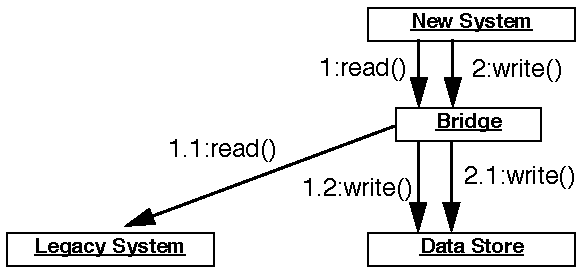
\includegraphics[width=0.75\textwidth]{MigrationBridge}
\caption{A Bridge helps you to transparently transfer data to the new system.}
\figlabel{MigrationBridge}
\end{center}
\end{figure}

Make a (data) bridge that will incrementally transfer data from the legacy system to the replacement system as new components are ready to take the data over from their legacy counterparts.

\subsubsection*{Steps}

\begin{bulletlist}
\item Identify legacy and replacement components that deal with the same logical data entities.

\item Implement a ``\ind{data bridge}'' which is responsible for redirecting \emph{read} requests from the new component to the legacy data source, if the data have not already been migrated. The bridge is responsible for any necessary data conversion. The new component should not be aware of the bridge.

\item Adapt the legacy component to redirect \emph{write} requests to the new component, so that the new data stay up-to-date.

\item When all the data have been transferred, remove the bridge and the legacy component.
\end{bulletlist}

\subsection*{Tradeoffs}

\subsubsection*{Pros}

\begin{bulletlist}
\item You can start using the new system without migrating all the legacy data.
\end{bulletlist}

\subsubsection*{Cons}

\begin{bulletlist}
\item A data bridge can be tricky to implement correctly if there is not a simple mapping between the legacy data and the new data.

\item Once some of the data has been transferred, it can be hard to go back.

\item The data bridge will add a performance overhead which may or may not be acceptable.
\end{bulletlist}

\subsubsection*{Difficulties}

\begin{bulletlist}
\item \emph{``Stepwise migration schemes have proven very effective in large, layered business systems. They are not common in let's say CAD applications that have check in /check out persistence and a tightly coupled and very woven object net.''} \cite{Kell00a}
\end{bulletlist}

\subsection*{Known Uses}

\index{Brodie, Michael}
\index{Stonebraker, Michael}
Brodie \& Stonebraker discuss much more thoroughly the use of data bridges and gateways in \emph{Migrating Legacy Systems} \cite{Brod95a}. 

\index{Keller, Wolfgang}
Keller in ``The Bridge to the New Town'' \cite{Kell00a} focusses more on the technical issue of migrating legacy data, and he points out numerous examples of the pattern successfully being applied.

There are many possible variants of this pattern, depending on whether the entire legacy system is to be replaced, or only a component, and whether users should be able to have access to both systems at the same time or not.

\subsection*{Rationale}

A bridge between the old and new systems allows you to let users start using features of the new system before it is complete. The bridge isolates the two systems from each other so that the new system can be developed according to a new architectural vision without influence from the legacy system.

\subsection*{Related Patterns}

A bridge helps you \patref{Migrate Systems Incrementally}{MigrateSystemsIncrementally} and thereby \patref{Build Confidence}{BuildConfidence}.

%=================================================================
%:PATTERN -- {Present the Right Interface}
\pattern{Present the Right Interface}{PresentTheRightInterface}

\emph{Also Known As:}  \ind{Semantic Wrapper} \cite{Ocal00a}, \ind{Sweeping it Under the Rug} \cite{Foot00a}

\intent{Wrap a legacy system to export the right abstractions, even if they are not reflected in the existing implementation.}

\subsection*{Problem}

How should the new target system access legacy services during the migration process?

\emph{This problem is difficult because:} 

\begin{bulletlist}
\item The target system is not yet complete so you must rely on legacy services during the migration. 

\item The legacy system does not present the interfaces you need for the target system.

\item Implementing new components directly in terms of legacy components will bias the target towards the legacy architecture and design.
\end{bulletlist}

\emph{Yet, solving this problem is feasible because:}

\begin{bulletlist}
\item You don't have to access the legacy services directly.
\end{bulletlist}

\subsection*{Solution}

Identify the abstractions that you want to have in the new system, and wrap up the old software to emulate the new abstractions.

\subsubsection*{Hints}

Consider, for example, a procedural graphics library that will be used within an object-oriented system. It will be too costly and time-consuming to reimplement the library in an object-oriented way. It would be easier to wrap it as a utility class (\ie as a class with static methods but no instances), but it would be wiser to write a slightly thicker wrapper that presents a truly object-oriented interface, but is implemented using the underlying procedural abstractions. In this way the new system will not be polluted by legacy abstractions. 

\subsection*{Tradeoffs}

\subsubsection*{Pros}

\begin{bulletlist}
\item It is easier to wean the target system from legacy services if they can use appropriate abstractions from the start.

\item You reduce the risk that the legacy design will adversely influence the new target.
\end{bulletlist}

\subsubsection*{Cons}

\begin{bulletlist}
\item The new interface may not be stable, so developers may be reluctant to use it.
\end{bulletlist}

\subsubsection*{Difficulties}

\begin{bulletlist}
\item It can be hard to resist the temptation to simply wrap the procedural abstractions as utility classes.
\end{bulletlist}

\subsection*{Known Uses}

\index{O'Callaghan, Alan}
Alan O'Callaghan \cite{Ocal00a} presents this pattern as ``\ind{Semantic Wrapper}'' briefly in the context of the \ind{ADAPTOR pattern language}, which addresses migration of large-scale business-critical legacy systems to object-oriented and component-based technology. 

\subsection*{Rationale}

\patref{Present the Right Interface}{PresentTheRightInterface} frees you from thinking in terms of the legacy design and makes it easier to consider alternative approaches.

\subsection*{Related Patterns}

\patref{Present the Right Interface}{PresentTheRightInterface} superficially resembles an \patpgref{Adapter}{Adapter}, since both use wrappers as their implementation technique. An \patref{Adapter}{Adapter}, however, adapts an incompatible interfaces to another interface expected by its clients. \patref{Present the Right Interface}{PresentTheRightInterface}, on the other hand, introduces a new, more suitable interface to a legacy component. 

Be sure to \patref{Deprecate Obsolete Interfaces}{DeprecateObsoleteInterfaces}. 

If the new interface implemented by the \patref{Present the Right Interface}{PresentTheRightInterface} is not stable, you should \patref{Distinguish Public from Published Interface}{DistinguishPublicFromPublishedInterface}.

%=================================================================
%:PATTERN -- {Distinguish Public from Published Interface}
\pattern{Distinguish Public from Published Interface}{DistinguishPublicFromPublishedInterface}

\emph{Also Known As:}  \ind{Published Interface} \cite{Ocal00a}

\intent{Facilitate parallel development by distinguishing unstable ``published interfaces'' from stable ``public interfaces''.}

\subsection*{Problem}

How do you enable migration from legacy interfaces to new target interfaces while the new interfaces are still under development?

\emph{This problem is difficult because:} 

\begin{bulletlist}
\item You want to enable migration to the new target system as early as possible.

\item You do not want to freeze the interfaces of new target components too early.

\item Changing the interface to a component that is widely used will slow down development.
\end{bulletlist}

\emph{Yet, solving this problem is feasible because:}

\begin{bulletlist}
\item You can control the status of the interfaces you provide.
\end{bulletlist}

\subsection*{Solution}

Distinguish between public interfaces of components that are available to the rest of the system, and unstable ``published'' interfaces of components that are available within a subsystem, but are not yet ready for prime time.

\subsubsection*{Hints}

Since ``published'' interfaces are not supported by any programming language, you may have to use naming conventions, or abuse other features to achieve the desired effect.

\begin{bulletlist}
\item In \ind{Java}, consider declaring such interfaces as \lct{protected}, or giving them package scope (undeclared). When the interfaces stabilize, you may redeclare them as being \lct{public}.

\item In \ind{C++}, consider declaring components with published interfaces \lct{private} or \lct{protected}, and declare as \lct{friends} the clients that are permitted to use them. When the interfaces stabilize, redeclare the components as \lct{public}, and delete the declarations of \lct{friends}.

\item In \ind{Smalltalk}, consider declaring categories of published components. Also consider declaring published message categories to distinguish stable and unstable messages.

\item Consider decorating the names of unstable components or interfaces to indicate their ``published'' status. When the component becomes public, rename it and patch all its clients or deprecate the version with the old name (\patref{Deprecate Obsolete Interfaces}{DeprecateObsoleteInterfaces}).
\end{bulletlist}

\subsection*{Tradeoffs}

\subsubsection*{Pros}

\begin{bulletlist}
\item Clients of published interfaces are aware that they are likely to change.
\end{bulletlist}

\subsubsection*{Cons}

\begin{bulletlist}
\item Identifying an interface as ``published'' is purely a matter of convention and discipline.

\item Promoting an interface from published to public entails a certain overhead for clients who should upgrade to the new interface.
\end{bulletlist}

\subsubsection*{Difficulties}

\begin{bulletlist}
\item Clients can be put in a bind: should they use an unstable published interface, or continue to use the legacy service?
\end{bulletlist}

\subsection*{Known Uses}

\ind{Published Interface} is another pattern of the \ind{ADAPTOR pattern language} \cite{Ocal00a}.

\subsection*{Rationale}

Clients are in a better position to evaluate the risk of using a component if they know its interface is declared to be ``published'' but not yet public.

\subsection*{Related Patterns}

When you \patref{Present the Right Interface}{PresentTheRightInterface} to a legacy component, the new interface may not be stable, so be careful to \patref{Distinguish Public from Published Interface}{DistinguishPublicFromPublishedInterface}. When the new interface stabilizes, or is substituted by a stable replacement component, the interface may become public.

Upgrading an interface to public may entail a change to the way it is accessed. Be sure to \patref{Deprecate Obsolete Interfaces}{DeprecateObsoleteInterfaces}.

%=================================================================
%:PATTERN -- {Deprecate Obsolete Interfaces}
\pattern{Deprecate Obsolete Interfaces}{DeprecateObsoleteInterfaces}

\emph{Also Known As:}  \ind{Deprecation} \cite{Stev98a}

\intent{Give clients time to react to changes to public interfaces by flagging obsolete interfaces as ``deprecated''.}

\subsection*{Problem}

How do you modify an interface without invalidating all the clients?

\emph{This problem is difficult because:} 

\begin{bulletlist}
\item Changing a public interface can break many clients.

\item Leaving an obsolete interface in place will make future maintenance more difficult.

\item Not all changes are for the better.
\end{bulletlist}

\emph{Yet, solving this problem is feasible because:}

\begin{bulletlist}
\item The old and the new interfaces can coexist for a period of time.
\end{bulletlist}

\subsection*{Solution}

Flag the old interface as being ``deprecated'', thereby notifying clients that it will almost certainly be removed in the next upcoming release.

\subsubsection*{Steps}

\begin{bulletlist}
\item You have determined that a public interface should be changed, but you do not want to break all clients. Implement the new interface, but ``deprecate'' the old one. The deprecation mechanism should inform clients that the interface has changed, and that a newer interface is recommended instead.

\item Evaluate to what extent the deprecated interface continues to be used, and whether it can be permanently retired. Consider removing it in a future release.

\item \ind{Java} supports deprecation as a language feature:
\begin{bulletlist}
\item Deprecate a feature by adding the tag \lct{@deprecated} to its javadoc documentation. The tag is not only recognized by the javadoc documentation generator, but the compiler will also generate compile-time warnings if code using deprecated features is compiled with the -deprecated option.
\end{bulletlist}

\item Other approaches are:

\begin{bulletlist}
\item Simply inform users in the documentation which interfaces are deprecated.

\item Move or rename the deprecated interface or component. Clients can continue to use them, but must adapt and recompile to continue to use the deprecated form.

\item Replace deprecated components by equivalent ones that generate run-time warnings or output warnings to a log file. 

\item Alternatively, consider configuring the programming environment or the deprecated components themselves to generate compile-time or link-time warnings.
\end{bulletlist}
\end{bulletlist}

\subsection*{Tradeoffs}

\subsubsection*{Pros}

\begin{bulletlist}
\item Clients do not have to immediately adapt to changes.

\item There is time to change your mind.
\end{bulletlist}

\subsubsection*{Cons}

\begin{bulletlist}
\item Clients are free to ignore deprecation.
\end{bulletlist}

\subsubsection*{Difficulties}

\begin{bulletlist}
\item It may be hard to track down all the clients of a deprecated component.

\item It can be hard to decide when to really retire a deprecated component.

\item If you want to keep the interface but change the semantics, you may need to introduce a new component and deprecate the old one. This can be the case if certain methods should now return default values instead of throwing exceptions (or vice versa).
\end{bulletlist}

\subsection*{Known Uses}

\index{Stevens, Perdita}
\index{Pooley, Rob}
Perdita Stevens and Rob Pooley identify \ind{Deprecation} as a common practice for managing evolving APIs in complex systems \cite{Stev98a}.

\subsection*{Rationale}

Deprecation gives you a window of time to evaluate the impact of a change.

%=================================================================
%:PATTERN -- {Conserve Familiarity}
\pattern{Conserve Familiarity}{ConserveFamiliarity}


\intent{Avoid radical changes that may alienate users.}

\subsection*{Problem}

How do you accomplish a major overhaul of a legacy system without disrupting the way users are used to getting their job done?

\emph{This problem is difficult because:} 

\begin{bulletlist}
\item The legacy system requires significant changes.

\item The users are not happy with the legacy system, but they understand it well.
\end{bulletlist}

\emph{Yet, solving this problem is feasible because:}

\begin{bulletlist}
\item You can migrate incrementally to a new solution.
\end{bulletlist}

\subsection*{Solution}

Introduce only a constant, relatively low number of changes between each new release.

\subsection*{Tradeoffs}

\subsubsection*{Pros}

\begin{bulletlist}
\item Users do not have to change their work habits too much between releases.
\end{bulletlist}

\subsubsection*{Difficulties}

\begin{bulletlist}
\item Sometimes radical change is necessary. It can be hard to migrate from a command-line interface to a GUI while conserving familiarity.
\end{bulletlist}

\subsection*{Rationale}

Too much change between releases increases the risk of hidden defects, and decreases the chance of user acceptance. 

\index{Lehman, Manny}
\index{Belady, Les}
Lehman and Belady's ``\ind{Law of Conservation of Familiarity}'' suggests that the incremental change between releases of a system stays roughly constant over time \cite{Lehm85a}. This is a relatively natural phenomenon because to do anything else introduces unnecessary risks.

\subsection*{Related Patterns}

To \patref{Conserve Familiarity}{ConserveFamiliarity} you must \patref{Migrate Systems Incrementally}{MigrateSystemsIncrementally}. \patref{Involve the Users}{InvolveTheUsers} to understand what changes will be acceptable. \patref{Prototype the Target Solution}{PrototypeTheTargetSolution} to evaluate the potential impact of changes.

%=================================================================
%:PATTERN -- {Use Profiler Before Optimizing}
\pattern{Use Profiler Before Optimizing}{UseProfilerBeforeOptimizing}


\intent{Avoid squandering reengineering effort on needless ``optimizations'' by verifying where the bottlenecks are.}

\subsection*{Problem}

When should you rewrite a clearly inefficient piece of code?

\emph{This problem is difficult because:} 

\begin{bulletlist}
\item When you are reengineering software, you are likely to encounter many naive algorithms in the legacy code.

\item It can be hard to predict what will impact performance, and you can lose a lot of time on pure supposition.

\item Optimized code is often more complex than simple, naive code.
\end{bulletlist}

\emph{Yet, solving this problem is feasible because:}

\begin{bulletlist}
\item There are tools to tell you where you may have a performance problem.
\end{bulletlist}

\subsection*{Solution}

Whenever you are tempted to optimize a ``clearly inefficient'' part of the system, first use a profiler to determine whether it is actually a bottleneck. 

Don't optimize anything unless your profiler tells you it will make a difference.

If you decide to go ahead, prepare benchmarks that will demonstrate the performance gains. 

\subsection*{Tradeoffs}

\subsubsection*{Pros}

\begin{bulletlist}
\item You do not waste time optimizing something that will not make a difference to overall performance.
\end{bulletlist}

\subsubsection*{Cons}

\begin{bulletlist}
\item Naive algorithms will survive longer in the system.
\end{bulletlist}

\subsection*{Rationale}

The performance improvement that you can gain by optimizing a bit of code depends on how much time the program, spends in that code in a typical run. A profiler will tell you how much time that is.

``\ind{Do it, then do it right, then do it fast}'' is a well-known aphorism that has been credited to many different sources. Very likely its origin is outside of the field of computer science. The rationale behind it is that you risk making a system complex and hard to maintain if you become preoccupied with performance issues too early. Instead, it is better to first find a solution that works, then clean it up once you understand it. Finally, if you can identify any important performance bottlenecks, that is the time to optimize just those parts that will make a difference.

As a corollary, it may even be a good idea to replace a bit of complex, ``optimized'' code by a simpler, ``naive'' solution, if that won't severely impact performance, but will make it easier to make other changes. 

\index{Davis, Alan}
See also Davis' discussion of ``\patref{Use Profiler Before Optimizing}{UseProfilerBeforeOptimizing}'' \cite{Davi95a}.

\subsection*{Related Patterns}

If you \patpgref{Refactor to Understand}{RefactorToUnderstand}, you will have started the second step to ``do it right."

%=============================================================
\ifx\wholebook\relax\else
   \bibliographystyle{alpha}
   \bibliography{scg}
   \end{document}
\fi
%=============================================================
